\documentclass{article}
\usepackage[a4paper,margin=1in,footskip=0.25in]{geometry}
\usepackage[polish,provide=*]{babel}
\usepackage{float,graphicx}
\usepackage[T1]{fontenc}
\usepackage{hyperref}
\usepackage{float}
\usepackage{multicol}
\graphicspath{./graphs/}

\title{Przewidywanie oczekiwanej długości życia w kraju, na podstawie wskaźników jakości życia}
\author{Patryk Łuszczek \\ 272707@student.pwr.edu.pl \\ MSiD Lab Wtorek 7.30 NP}

\date{18 maja 2024}

\begin{document}

\maketitle
\pagebreak

\tableofcontents
\pagebreak

\section{Wprowadzanie}
\subsection{Opis problemu}
Rozpatrywanym problemem jest wpływ różnych wskaźników jakości życia na oczekiwaną długość życia w danym kraju.
Analiza tych wskaźników pozwala na zrozumienie, które z nich mają największy wpływ na zdrowie i jakość życia mieszkańców.
\subsection{Cel}
Celem projektu jest stworzenie modelu, który na podstawie parametrów związanych z jakością życia w danym kraju, będzie w stanie przewidzieć oczekiwaną długość życia w tym kraju.
Wybór konkretnych wskaźników został dokonany z uwzględnieniem ich potencjalnego wpływu na zdrowie i jakość życia mieszkańców.
Dla przykładu wskaźniki takie jak GNI per capita oraz HDI bezpośrednio odzwierciadlającymi jakość życia, poziom rozwoju ekonomicznego
i społecznego kraju. Z kolei, wskaźniki takie jak konsumpcja alkoholu per capita, cena najtańszych papierosów czy odsetek ubóstwa
mogą być powiązane z zachowaniami wpływającymi na zdrowie obywateli. \\ \\
Parametrami, które zostały wybrane do analizy są:
\begin{itemize}
    \item Populacja kraju,
    \item Konsumpcja alkoholu per capita,
    \item Ilość łóżek szpitalnych na 10 000 osób,
    \item Miejsce w rankingu HDI,
    \item GNI per capita,
    \item Zagęszczenie szpitali,
    \item Wskaźnik ICT - stopień zaawansowania technologicznego kraju,
    \item Nutrition Governance Score - wskaźnik oceniający jakość zarządzania publicznego w obszarze polityki żywieniowej oraz dostępu do zdrowej żywności w kraju,
    \item Cena najtańszych papierosów w dolarach,
    \item Odsetek ubóstwa,
    \item Średnia cena 500 ml piwa,
    \item Odsetek osób korzystających z zewnętrznych toalet,
    \item Wydatki na służbę zdrowia jako procent PKB,
\end{itemize}

\pagebreak

\section{Zbiór danych}
\subsection{Źródło oraz pozyskanie danych}
Dane wykorzystane do rozwiązania problemu zostały pobrane za pomocą publicznego \href{https://www.who.int/data/gho/info/gho-odata-api}{GHO OData API} 
udostępnionego przez \href{https://www.who.int}{World Health Organization}. Z wykorzystaniem tego API można pobrać dane związane z różnymi aspektami zdrowia publicznego, takimi jak
wskaźniki średniej długości życia, dostępności służby zdrowia czy odsetek zakażeń różnymi chorobami. API pozwala na formatowanie danych w formacie JSON, co
znacząco ułatwia ich przetwarzanie. W celu pozyskania danych z API, został napisany skrypt w języku Python, który pozwala na wybór interesujących nas wskaźników, a następnie formatuje dane
w przyjazny dla dalszej analizy sposób. W związku z częstą zawodnością API, poszczególne framgenty zbioru są zapisywane w plikach JSON, dzięki czemu mogą bez problemu zostać wczytane
do analizy w przyszłości bez konieczności polegania na dostępności serwisu.
\subsection{Wstępne przetwarzanie}
W związku z niewielką ilością danych, związanych z ograniczoną liczbą krajów, są one niezwykle wrażliwe na wszelkie modyfikacje.
Kraje nieposiadające wartości docelowej (oczekiwanej długości życia) zostały usunięte ze zbioru, ponieważ nie byłyby przydatne do uczenia modelu.
Odestek brakujących wartości dla pozostałych wskaźników prezentuje się następująco

\begin{figure}[H]
    \label{fig:missing_values}
    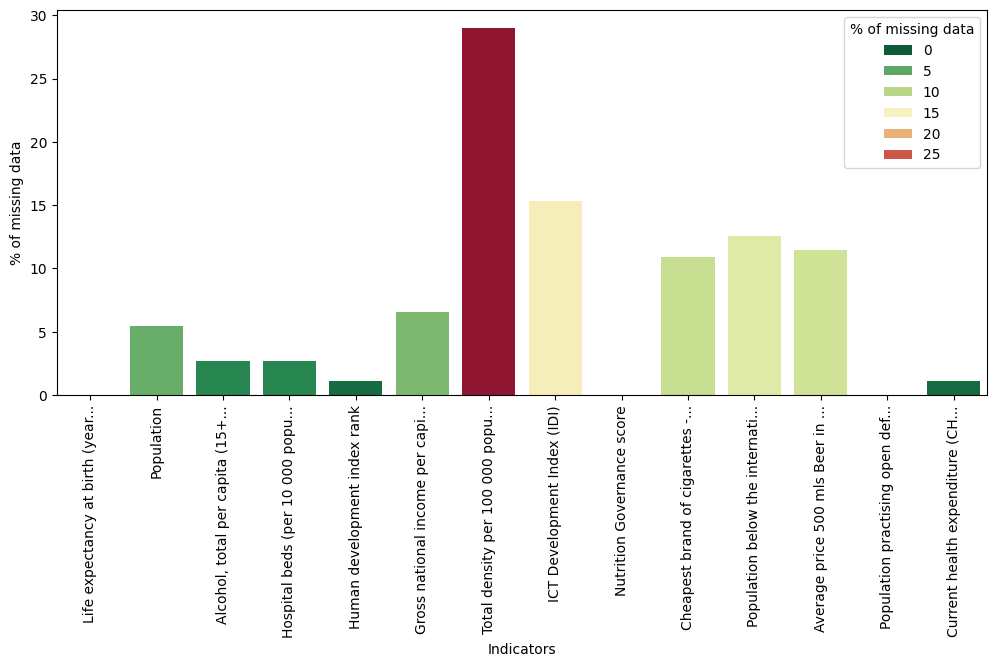
\includegraphics[width=\textwidth]{graphs/missing_values.png}
    \caption{\% brakujących wartości dla poszczególnych wskaźników}
    \centering
\end{figure}

Znacząca liczba krajów nie posiada danych dotyczących zagęszczenia szpitali, co może wpłynąć na jakość modelu. W związku z tym dane te zostały usunięte z dalszej analizy.
Dodatkowo, populacja kraju z logicznego punktu widzenia nie powinna mieć wpływu na oczekiwaną długość życia, dlatego również została wykluczona z dalszej analizy.
Wiersze z brakującymi danymi dotyczącymi spożycia alkoholu, łóżek szpitalnych oraz rankingu HDI zostały wypełnione wartościami średnimi dla danego wskaźnika. 
Ostatecznie wiersze z brakującymi danymi w którejkolwiek z kolumn zostały wykluczone z analizy. Finalnie zbiór danych składa się z 12 kolumn (wskaźników) oraz 115 wierszy (krajów).

\pagebreak
\subsection{Analiza eksploracyjna}
\begin{enumerate}
    \item Cel - oczekiwana długość życia
    \begin{itemize}
        \item Rozkład: 
        \begin{figure}[H]
                \label{fig:life_expectancy_distribution}
                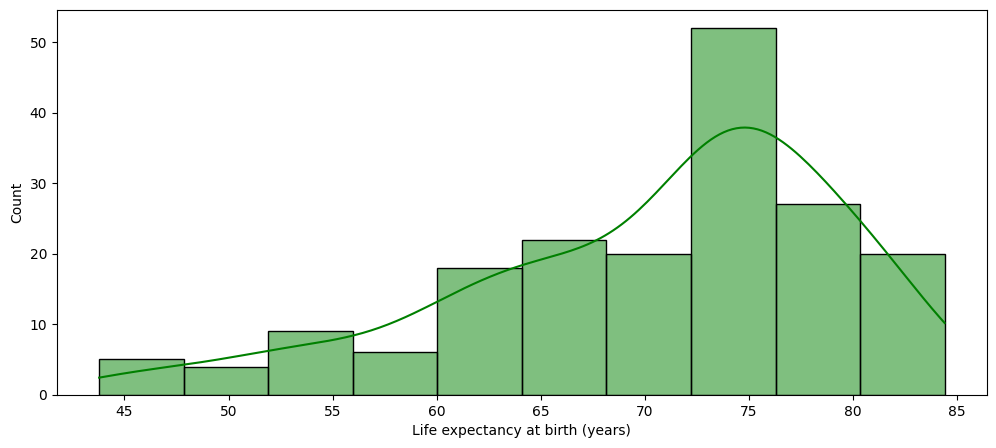
\includegraphics[width=\textwidth]{graphs/life_expecatancy_buckets.png}
                \caption{Rozkład}
                \centering
        \end{figure}
        \item Przykładowe wartości:
        \begin{figure}[H]
                \label{fig:sample_life_expectancy}
                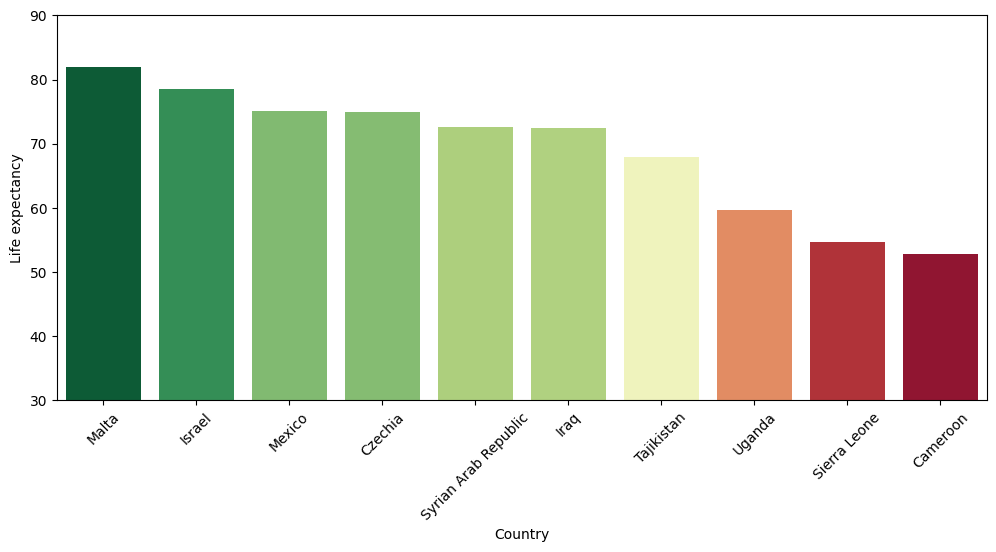
\includegraphics[width=\textwidth]{graphs/life_expectancy_sample.png}
                \caption{Przykładowe wartości}
                \centering
        \end{figure}
    \end{itemize}
    \pagebreak
    \item Mapa korelacji
        \begin{figure}[H]
                \label{fig:correlation_map}
                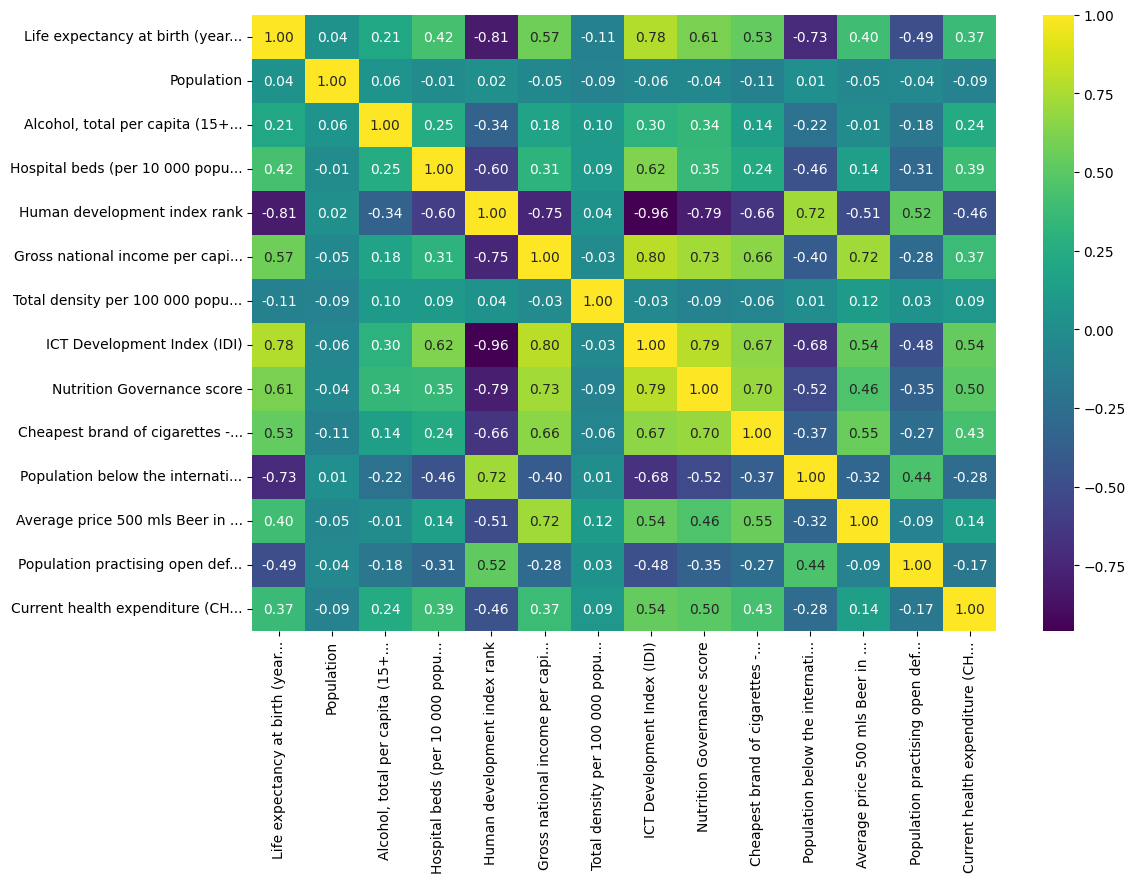
\includegraphics[scale=0.52]{graphs/corr_matrix.png}
                \caption{Mapa korelacji}
                \centering
        \end{figure}

    Dzięki mapie korelacji można dostrzec zależności między poszczególnymi wskaźnikami. 
    Analiza wykresu pozwala na stwierdzenie, że największy wpływ na oczekiwaną długość życia mają wskaźniki takie jak: 
    HDI, GNI, odsetek ubóstwa oraz Nutrition Governance Score. Dodatkowo można zauważyć, że wskaźnik gęstości szpitali jak i populacja nie mają wpływu na oczekiwaną długość życia,
    więc założenie o ich całkowitym wykluczeniu analizy było słuszne.

    \item Zależność długości życia od poszczególnych wskaźników
    
    Wizualizacja każdej zależności ułatwia znalezienie potencjalnych outlierów, które mogą wpłynąć na jakość modelu.
    W rozpatrywanych danych nie znaleziono wartości znacząco odstających od reszty. Jest to związane z 
    faktem, że dane zostały dobrane ręcznie.
    Nałożenie na wykresy krzywej regresji pozwala na zauważenie zależności między wskaźnikami, a oczekiwaną długością życia.
    Niektóre wskaźniki nie wykazują tak oczywistej zależności, co sugeruje, 
    że niektóre z nich mogą mieć mniejszy wpływ na oczekiwaną długość życia w kraju.
    \begin{figure}[H]
        \begin{minipage}[t]{0.48\textwidth}
            \label{fig:alcohol_consumption}
            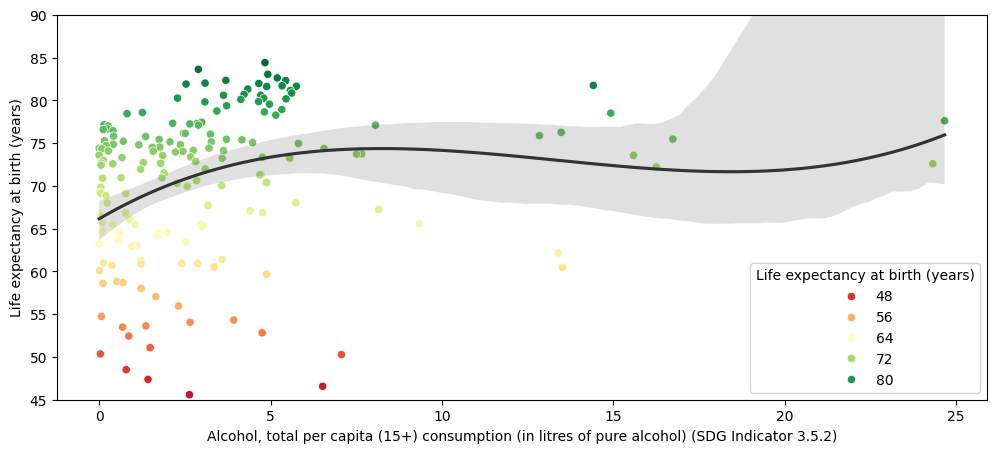
\includegraphics[width=\textwidth]{graphs/alcohol_consumption.png}
            \caption{Zależność długości życia od spożycia alkoholu}
            \centering
        \end{minipage}
        \hfill
        \begin{minipage}[t]{0.48\textwidth}
            \label{fig:hospital_beds}
            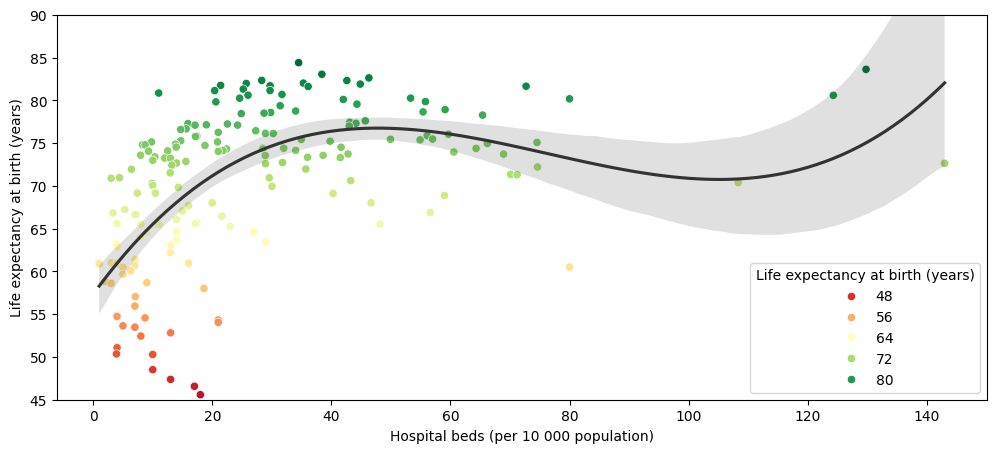
\includegraphics[width=\textwidth]{graphs/hospital_beds.png}
            \caption{Zależność długości życia od liczby łóżek szpitalnych na 10 000 osób}
            \centering
        \end{minipage}
    \end{figure}

    \begin{figure}[H]
        \begin{minipage}[t]{0.48\textwidth}
            \label{fig:hdi_rank}
            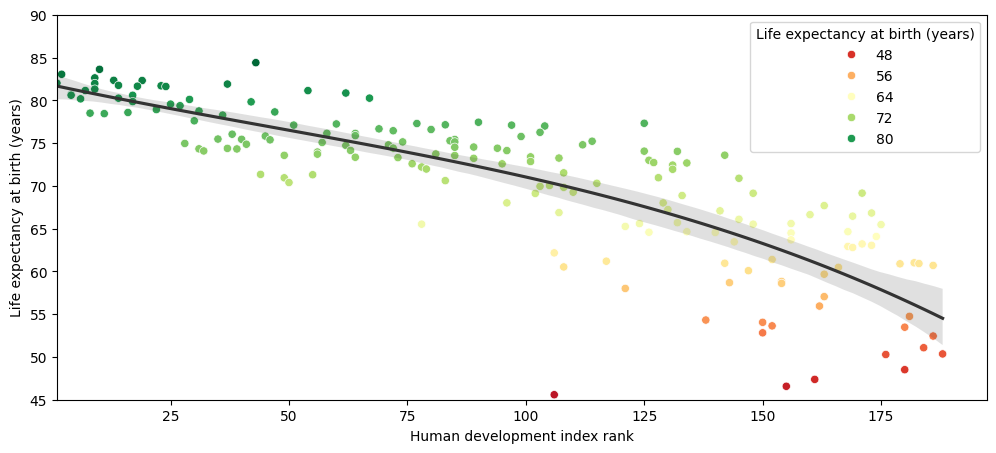
\includegraphics[width=\textwidth]{graphs/hdi_rank.png}
            \caption{Zależność długości życia od miejsca w rankingu HDI}
            \centering
        \end{minipage}
        \hfill
        \begin{minipage}[t]{0.48\textwidth}
            \label{fig:gni}
            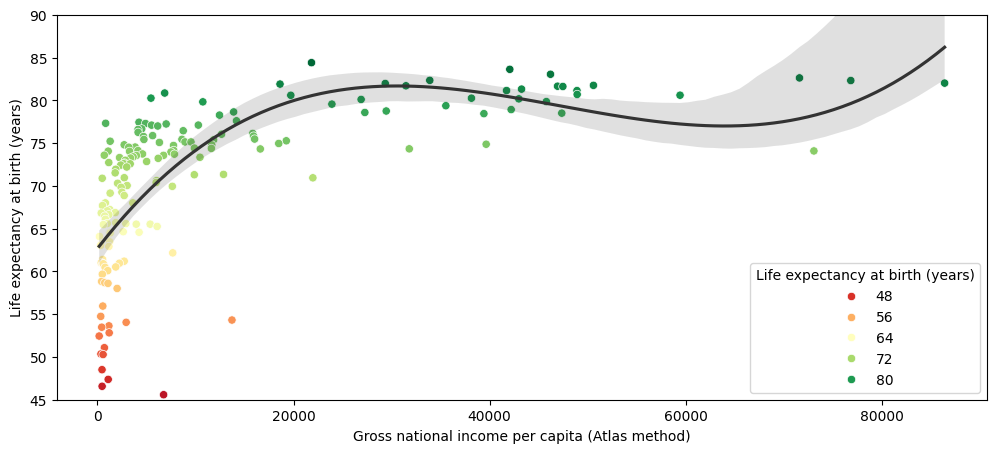
\includegraphics[width=\textwidth]{graphs/gni.png}
            \caption{Zależność długości życia od GNI per capita}
            \centering
        \end{minipage}
    \end{figure}

    \begin{figure}[H]
        \begin{minipage}[t]{0.48\textwidth}
            \label{fig:ict}
            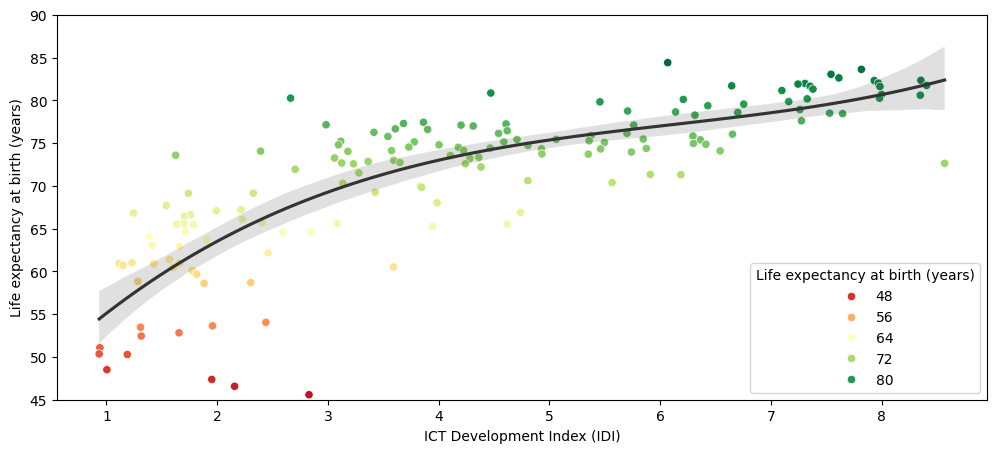
\includegraphics[width=\textwidth]{graphs/ict.png}
            \caption{Zależność długości życia od wskaźnika ICT}
            \centering
        \end{minipage}
        \hfill
        \begin{minipage}[t]{0.48\textwidth}
            \label{fig:nutrition}
            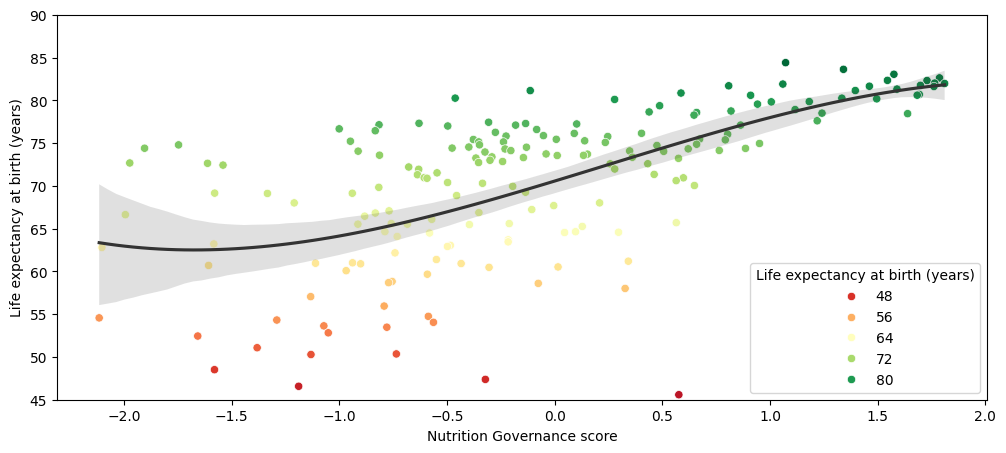
\includegraphics[width=\textwidth]{graphs/ngs.png}
            \caption{Zależność długości życia od Nutrition Governance Score}
            \centering
        \end{minipage}
    \end{figure}

    \begin{figure}[H]
        \begin{minipage}[t]{0.48\textwidth}
            \label{fig:cigarettes}
            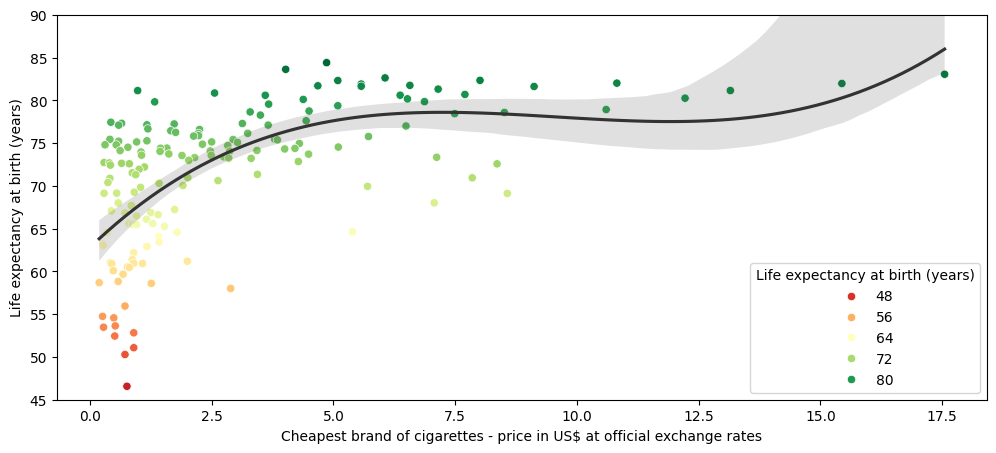
\includegraphics[width=\textwidth]{graphs/cigarettes.png}
            \caption{Zależność długości życia od ceny najtańszych papierosów w dolarach}
            \centering
        \end{minipage}
        \hfill
        \begin{minipage}[t]{0.48\textwidth}
            \label{fig:poverty}
            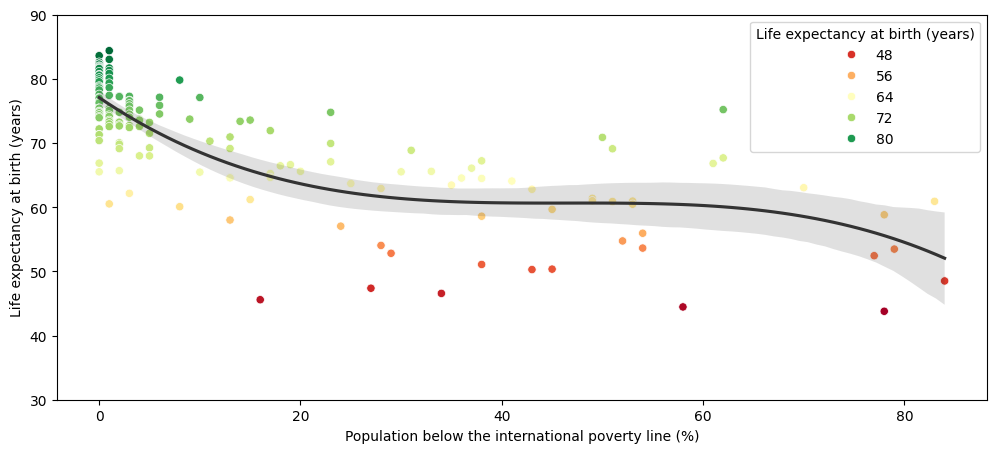
\includegraphics[width=\textwidth]{graphs/poverty.png}
            \caption{Zależność długości życia od odsetka ubóstwa}
            \centering
        \end{minipage}
    \end{figure}

    \begin{figure}[H]
        \begin{minipage}[t]{0.48\textwidth}
            \label{fig:beer}
            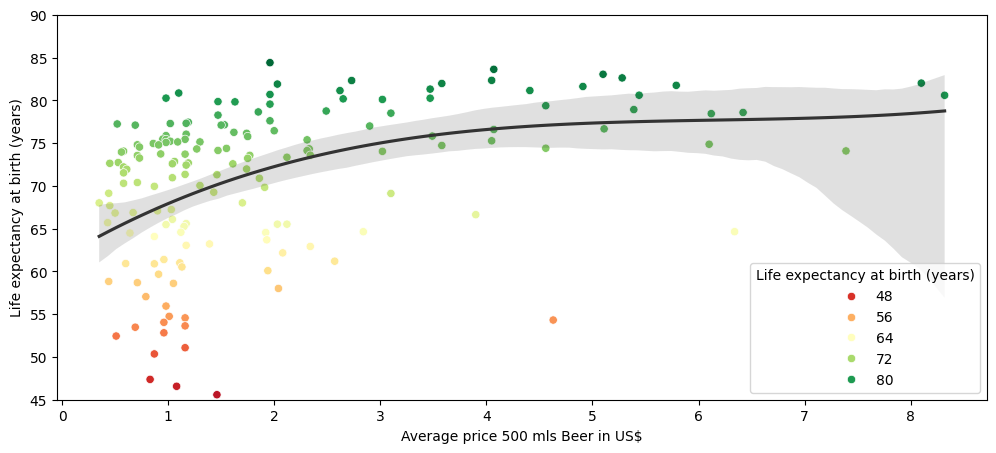
\includegraphics[width=\textwidth]{graphs/beer.png}
            \caption{Zależność długości życia od średniej ceny 500ml piwa}
            \centering
        \end{minipage}
        \hfill
        \begin{minipage}[t]{0.48\textwidth}
            \label{fig:toilets}
            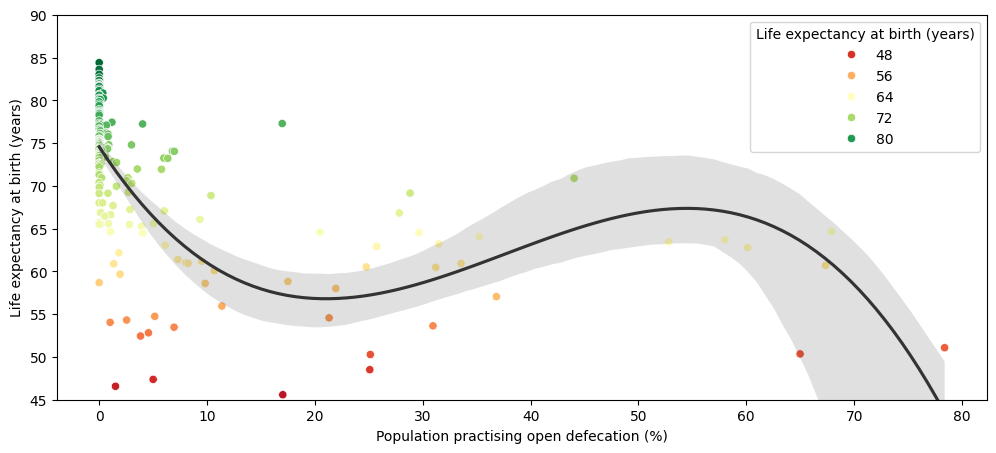
\includegraphics[width=\textwidth]{graphs/open_defecation.png}
            \caption{Zależność długości życia od spożycia alkoholu}
            \centering
        \end{minipage}
    \end{figure}

    \begin{figure}[H]
        \begin{minipage}[t]{0.48\textwidth}
            \label{fig:che}
            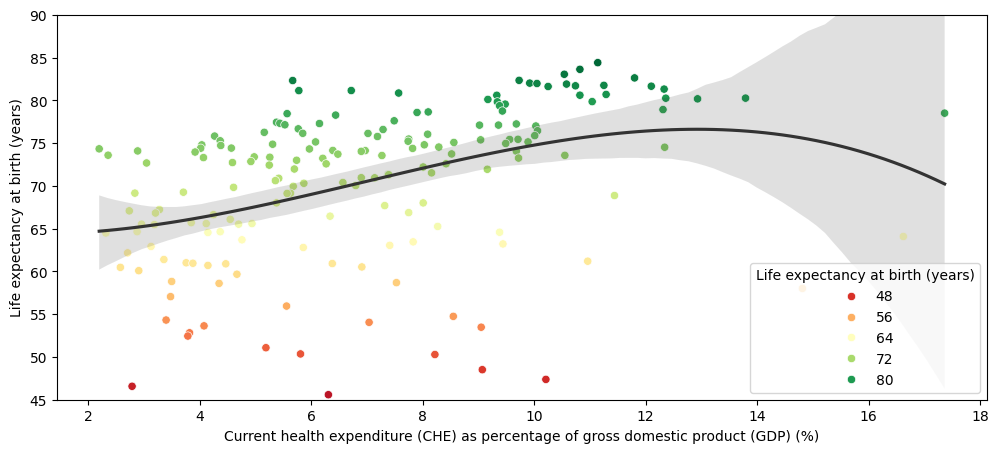
\includegraphics[width=\textwidth]{graphs/che.png}
            \caption{Zależność długości życia od wydatków na służbę zdrowia jako procent PKB}
            \centering
        \end{minipage}
    \end{figure}
\end{enumerate}

\section{Eksperymenty}

\subsection{Przygotowanie danych}
W celu przygotowania danych do uczenia modelu znormalizowano wartości wszystkich wskaźników, 
aby uniknąć problemów związanych z różnicą w skali wartości. Przykładowo wartości wskaźnika GNI per capita są rzędu $10^{4}$, 
podczas gdy wartości wskaźnika Nutrition Governance Score mieszczą się w przedziale $[-2,2]$.

\subsection{Wybór modelu}
\begin{multicols}{2}
W celu wybrania najlepszego modelu przetestowano kilka różnych modeli z bibilioteki scikit-learn obsługujących problem regresji. 
Modele zostały przetestowane z domyślnymi hiperparametrami, a następnie wybrano najlepszy model na 
podstawie jakości predykcji mierzonej za pomocą błędu średniokwadratowego (MSE),
średniego błędu bezwzględnego (MAE) oraz współczynnika determinacji $R^{2}$.
Metryka MSE mierzy średnią kwadratów różnicy między wartościami przewidywanymi, a rzeczywistymi penalizując duże błędy.
MSA mierzy średnią wartość bezwzględną różnicy między wartościami przewidywanymi, a rzeczywistymi, natomiast $R^{2}$ mierzy jak dobrze model przewiduje zmienność danych.
Użycie tych metryk pozwala na wszechstronne porównanie modeli, ponieważ każda z nich mierzy cechy modelu z innej perspektywy.
Modele, które zostały przetestowane to: Linear Regression, Ridge, Lasso, Random Forest Regressor, 
Decision Tree Regressor, Gradient Boosting Regressor oraz Elastic Net.
Test modeli przeprowadzono na zbiorze danych, który został losowo podzielony na zbiór 
treningowy i testowy w stosunku 80/20 oraz został powtórzony 250 razy, aby uzyskać uśrednione wyniki.
Z przperowadzonych badań wynika, że najlepszym modelem z podstawowymi hiperparametrami jest Ridge, który uzyskał najniższy błąd średniokwadratowy, 
najniższy średni błąd bezwzględny oraz najwyższy współczynnik $R^{2}$.
Oprocz tego modelu do dalszych badań wybrano również Random Forest Regressor oraz Grandient Boosting Regressor, 
które również uzyskały dobre wyniki, ale do optymalnego działania wymagają doboru odpowiednich hiperparametrów.
\begin{figure}[H]
    \label{fig:models_comparison}
    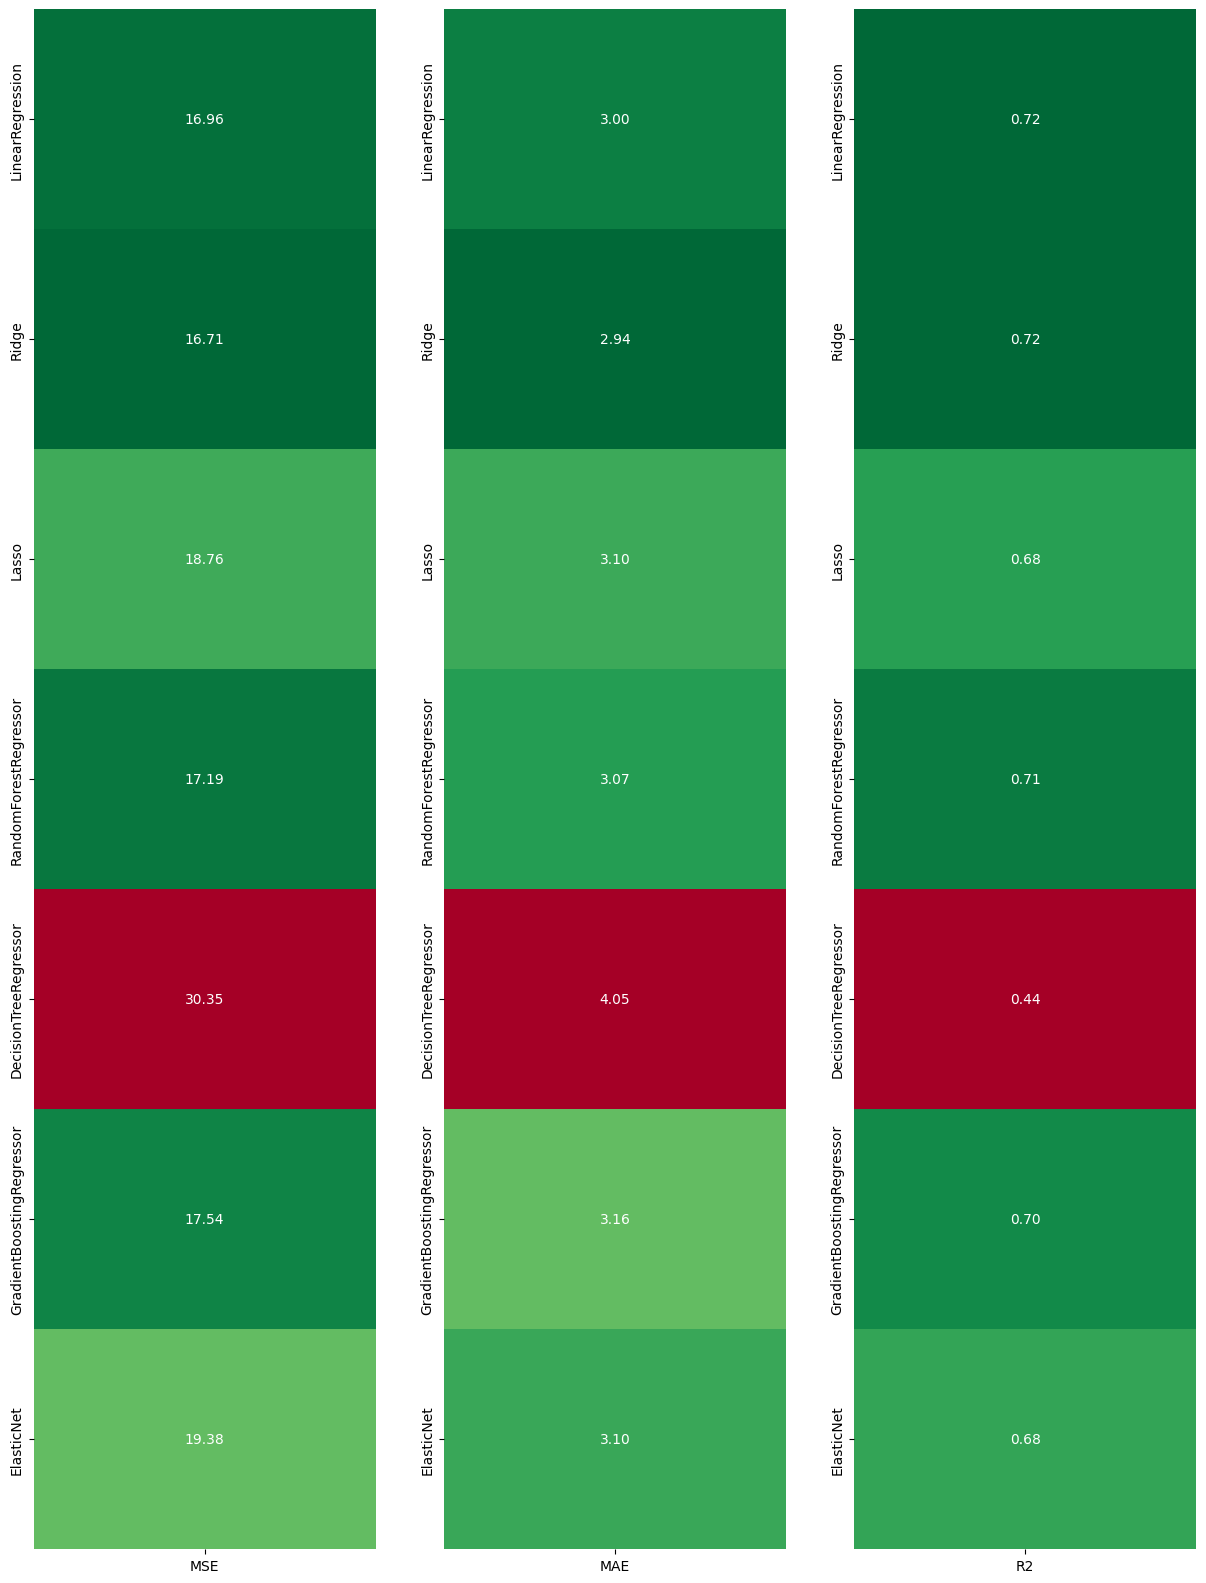
\includegraphics[scale=0.25]{graphs/all_models_comparsion.png}
    \caption{Porównanie modeli}
    \centering
\end{figure}
\end{multicols}

\subsection{Optymalizacja hiperparametrów}
Kolejnym krokiem jest znalezienie optymalnych hiperparametrów dla rozpatrywanych modeli. W tym celu została wykorzystana metoda Grid Search,
która pozwala na przetestowanie wielu kombinacji hiperparametrów, a następnie wybranie najlepszej z nich.
Każda z kombinacji została przetestowana na tym samym zbiorze danych, który został podzielony na zbiór treningowy oraz testowy w stosunku 80/20.
\subsubsection{Ridge}
Ridge jest modelem, który  do klasycznej regresji dodaje regularycję L2, co pozwala na uniknięcie overfittingu.
W przypadku tego modelu optymalizowano parametr \textit{alpha}, który określa siłę regularyzacji oraz parametr \textit{solver}, który określa algorytm optymalizacyjny. \\ \\
Wartościami parametrów wśród których przeprowadzono poszukiwania optymalnych wartości były: \\
\textit{alpha} $= [0.5, 1, 2, 5]$, \\
\textit{solver} $= ['auto', 'svd', 'cholesky', 'lsqr', 'sparse\_cg', 'sag', 'saga']$. \\
Wynikami optymalizacji są wartości \textit{alpha} $= 2$ oraz \textit{solver} $= 'saga'$.

\subsubsection{Random Forest Regressor}
Random Forest Regressor jest modelem, który składa się z wielu drzew decyzyjnych, a wynik predykcji jest średnią predykcją wszystkich drzew.
Model ten może służyć do rozwiązywania problemów regresji jak i klasyfikacji, co czyni go bardzo uniwersalnym.
Parametrami drzewa, które zostały objęte optymalizacją były: n\_estimators - liczba drzew w lesie, min\_samples\_split - minimalna liczba próbek wymagana do podziału węzła, 
min\_samples\_leaf - minimalna liczba próbek wymagana do utworzenia liścia, max\_features - liczba cech branych pod uwagę przy poszukiwaniu najlepszego podziału. \\ \\
Wartościami parametrów wśród których przeprowadzono poszukiwania optymalnych wartości, były: \\
\textit{n\_estimators} $= [5, 10, 25, 50]$, \\
\textit{min\_samples\_split} $= [5, 10, 15]$, \\
\textit{min\_samples\_leaf} $= [1, 3, 5]$, \\
\textit{max\_features} $= [0.2, 'sqrt', 'log2', 1]$.\\
Wynikami optymalizacji są wartości: \\
n\_estimators $= 5$, \\
min\_samples\_split $= 10$, \\
min\_samples\_leaf $= 3$, \\ 
max\_features $= 0.2$. \\


\subsubsection{Gradient Boosting Regressor}
Gradient Boosting Regressor jest jednym z popularniejszych modeli wykorzystywanych do uczenia maszynowego.
Model ten składa się z wielu słabych modeli - drzew decyzyjnych, które są dodawane do modelu w taki sposób, aby zminimalizować błąd predykcji.
Oprócz parametrów wymienionych w przypadku Random Forest Regressor, model ten posiada również parametr learning\_rate, który określa jak szybko model ma się uczyć. \\ \\
Parametrami, wśród których przeprowadzono poszukiwania optymalnych wartości, były: \\
\textit{n\_estimators} $= [125,150,200,300]$, \\
\textit{min\_samples\_split} $= [2, 5, 10]$, \\
\textit{min\_samples\_leaf} $= [1, 3, 5]$, \\
\textit{max\_features} $= [0.2, 'sqrt', 'log2', 1]$, \\
\textit{learning\_rate} $= [0.05, 0.075,0.1,0.15]$. \\
Wynikami optymalizacji są wartości:\\
n\_estimators $= 300$, \\
min\_samples\_split $= 10$, \\
min\_samples\_leaf $= 3$, \\
max\_features $= 0.2$, \\
learning\_rate $= 0.15$. \\

\pagebreak

\section{Wyniki}
\subsection{Porównanie modeli}
W wyniku optymalizacji hiperparametrów powstały modele, które uzyskały lepsze wyniki niż modele z domyślnymi hiperparametrami.
Metryki jakości modeli, które zostały wykorzystane do porównania to: błąd średniokwadratowy (MSE), średni błąd bezwzględny (MAE) oraz współczynnik determinacji $R^{2}$.
\begin{figure}[H]
    \label{fig:models_comparison_optimized}
    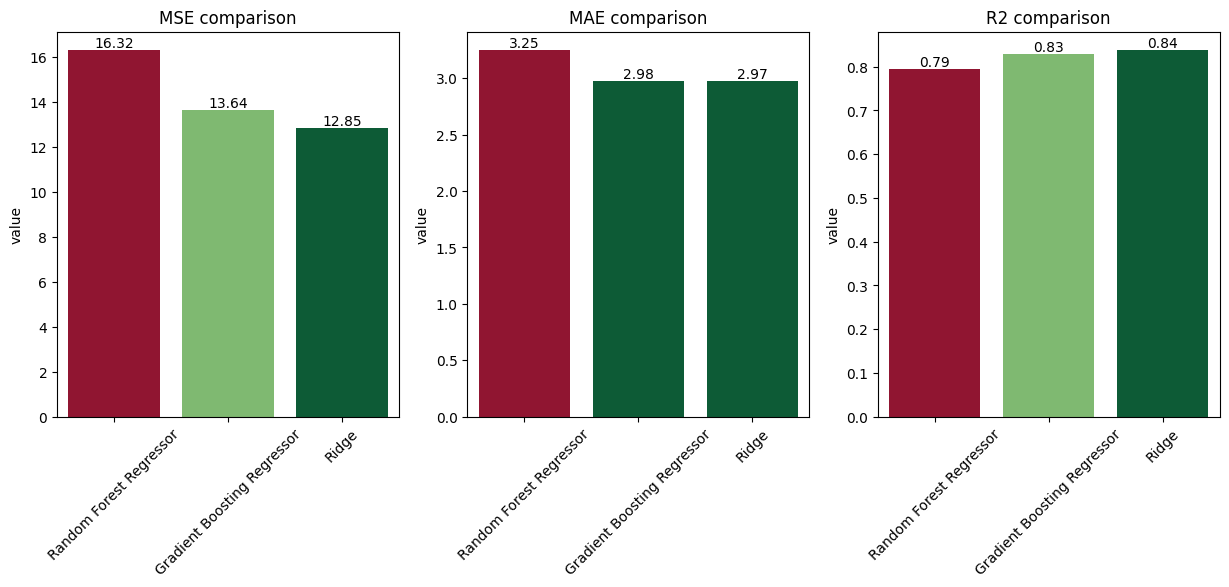
\includegraphics[width=\textwidth]{graphs/optimized_comparsion.png}
    \caption{Porównanie zoptymalizowanych modeli}
    \centering
\end{figure}
Modelem z najlepszymi wynikami jest Ridge Regression, który uzyskał najniższy błąd średniokwadratowy, średni błąd bezwzględny, oraz najwyższy współczynnik $R^{2}$.
Natomiast Grandient Boosting Regressor uzyskał bardzo zbliżone wyniki do Ridge Regression, co czyni go równie dobrym modelem do przewidywania oczekiwanej długości życia w kraju.
Najgorzej wypadł Random Forest Regressor, który uzyskał najwyższy błąd średniokwadratowy, średni błąd bezwzględny oraz najniższy współczynnik $R^{2}$. 
Pomimo uzyskania gorszych wyników model ten nadal jest w stanie przewidywać oczekiwaną długość życia z dużą dokładnością.

\subsection{Ważność cech dla Gradient Boosting Regressor}

Gradient Boosting Regressor jest modelem, który buduje kolejne drzewa decyzyjne na podstawie poprzednich drzew.
Zaletą tego modelu jest możliwość uzyskania informacji dotyczącej ważności poszczególnych cech dla modelu w procesie budowania drzewa.

\begin{figure}[H]
    \label{fig:feature_importance}
    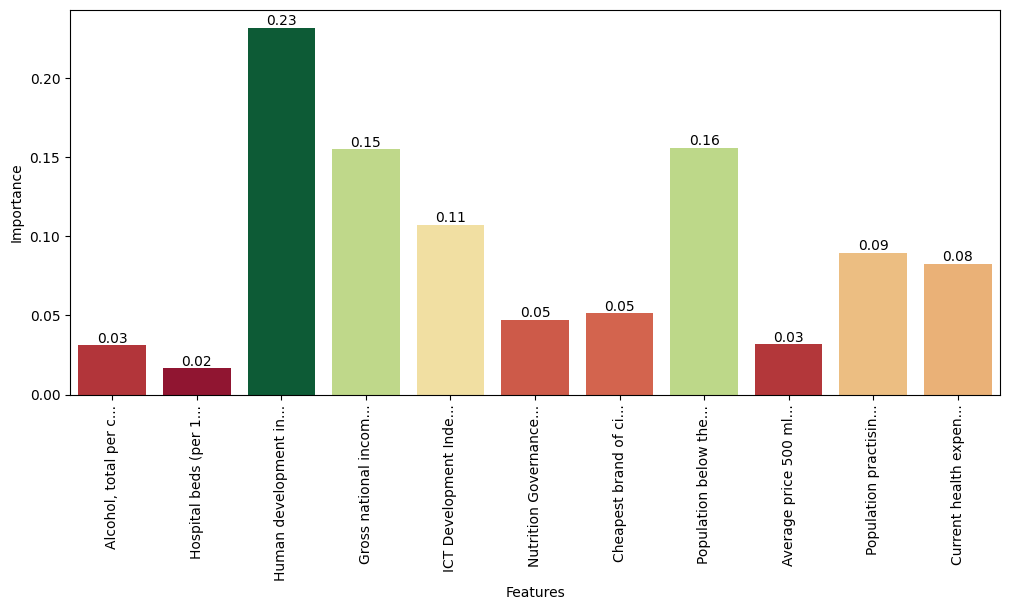
\includegraphics[width=\textwidth]{graphs/features_importance.png}
    \caption{Ważność cech dla Gradient Boosting Regressor}
    \centering
\end{figure}

Analiza ważności cech pozwala na stwierdzenie, że największy wpływ na oczekiwaną długość życia ma wskaźnik HDI (w tym przypadku miejsce w rankingu), co potwierdza wyniki analizy korelacji.
Kolejnymi ważnymi cechami są GNI per capita, odsetek ubóstwa oraz wskaźnik ICT. Pozostałe cechy mają nieco mniejszy wpływ (poniżej 10\%) na
szacowanie wartości docelowej. Przykładowo wskaźnik konsumpcji alkoholu per capita, cena najtańszych papierosów oraz
średnia cena 500 ml piwa mają marginalny wpływ na oczekiwaną długość. Wskaźnik ilości łóżek szpitalnych, choć mógłby wydawać 
się istotny, ma niewielki wpływ na wyniki.

\subsection{Przywidywanie, a rzeczywista wartość}

Porównanie predykcji z rzeczywistymi wartościami oczekiwanej długości dla każdego z modeli.

\begin{figure}[H]
    \label{fig:predictions_vs_real}
    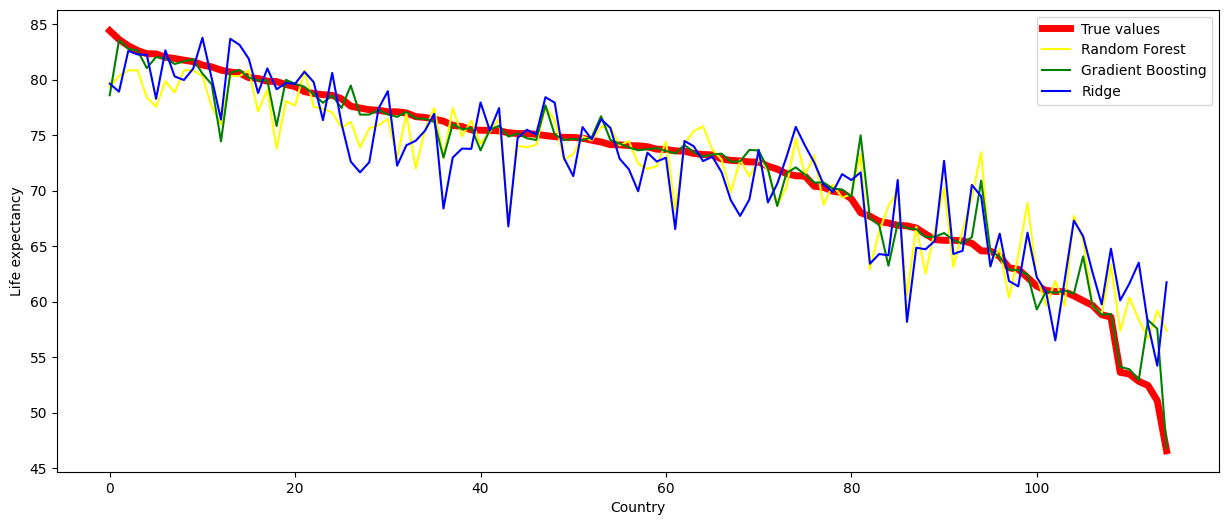
\includegraphics[width=\textwidth]{graphs/true_prediction.png}
    \caption{Porównanie predykcji z rzeczywistymi wartościami}
    \centering
\end{figure}

\pagebreak

Przywidywana wartość dla wybranych krajów:
\begin{multicols}{2}
    \begin{figure}[H]
        \label{fig:prediction_poland}
        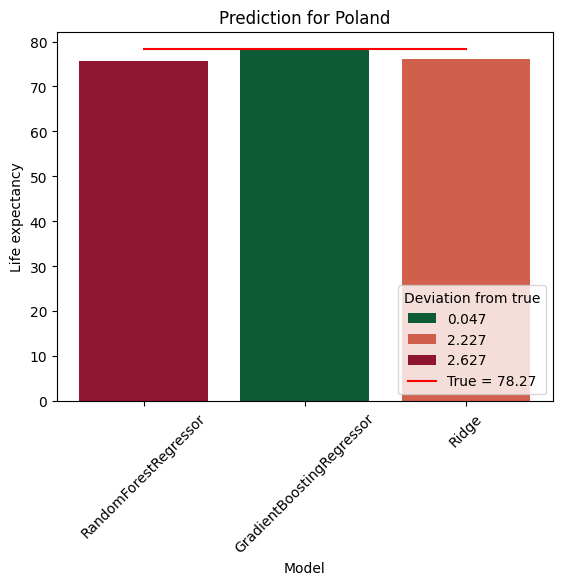
\includegraphics[scale=0.5]{graphs/pred_poland.png}
        \caption{Przewidywana wartość dla Polski}
        \centering
    \end{figure}
    \begin{figure}[H]
        \label{fig:prediction_japan}
        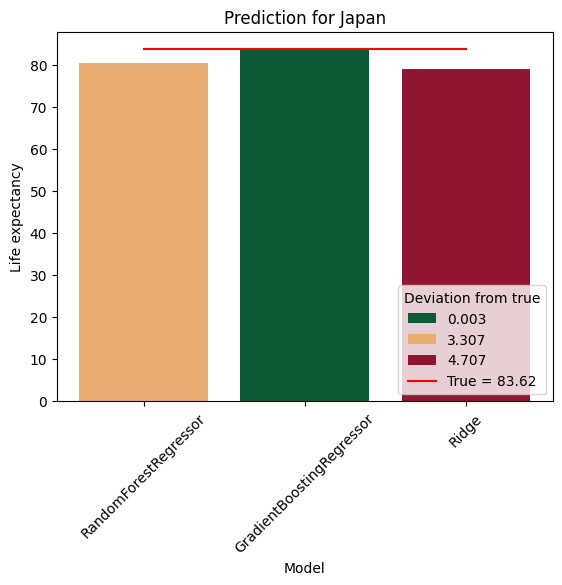
\includegraphics[scale=0.5]{graphs/pred_japan.png}
        \caption{Przewidywana wartość dla Japonii}
        \centering
    \end{figure}
    \begin{figure}[H]
        \label{fig:pred_thailand}
        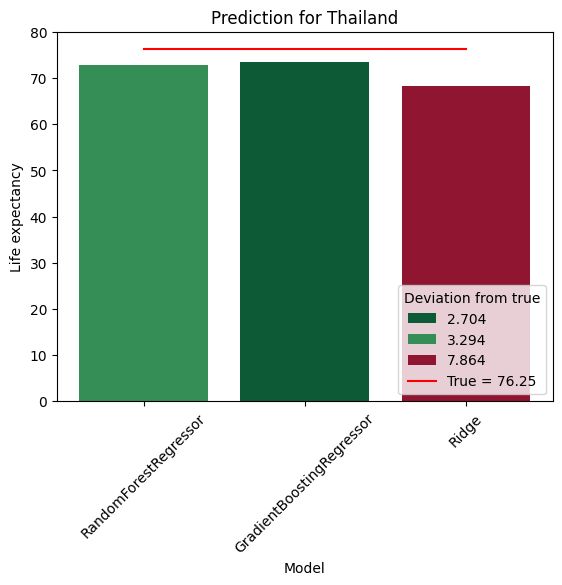
\includegraphics[scale=0.5]{graphs/pred_thailand.png}
        \caption{Przewidywana wartość dla Tajlandi}
        \centering
    \end{figure}
\end{multicols}

\section{Wnioski}
Zgodnie ze wstępną analizą danych zobserowano wysoką zależność między wskaźnikiem HDI, a oczekiwaną długością życia w kraju.
Z logicznego punktu widzenia kraje o wyższym HDI są w stanie zapewnić swoim obywatelom lepszą opiekę zdrowotną i generalnie lepsze warunki życia,
co przykłada się na większej średnia długość życia obywateli tych krajów. Z drugiej strony kraje słabo rozwinięte o niskim HDI mają mniejsze szanse na zapewnienie swoim obywatelom
dogodnych warunków życia, co skutkuje krótszą średnią długością życia.
Podobnie wysoka zależność została zaobserwowana dla wskaźników GNI per capita, odsetku ubóstwa oraz wskaźnika ICT, które są w pewnym
stopniu powiązane z HDI, co można było zauważyć we wczesnym etapie analizy na mapie korelacji.
Pozostałe wskaźniki charakteryzują się mniejszym wpływem na proces trenowania modeli, ale ich obecność pozwala na
uzyskanie dokładniejszych predykcji.

Zaskakująco mały wpłw na ostateczny wynik ma wskaźnik dotyczący ilości łóżek szpitalnych na 10 000 osób. 
Wynik ten może być spowodowany faktem, że ilość łóżek szpitalnych nie musi być jednocześnie powiązana
z jakością opieki zdrowotnej w danym kraju.

Mimo małego zbioru danych udało się uzyskać dość dokładne modele, których
wpółczynniki determinacji $R^{2}$ wahają się w granicach 80\%, co oznacza, że modele są w stanie przewidzieć
oczekiwaną długość życia z zaskakująco dużą dokładnością. Powodem tak dobrych wyników jest zdecydowanie
dobry dobór wskaźników, a przede wszystkim uwzględnienie wskaźników takich jak HDI, GNI per capita oraz odsetek ubóstwa,
które w logiczny sposób wpływają na jakość życia w danym kraju.
\end{document}